The method presented in this article has been implemented in a tool, called \textbf{Lyon}, written in OCaml. Given a graph transformation system $\mathcal{R}$ and a natural number, the tool automatically determines if there exists a suitable weighted graph with $n$ nodes without multiedges proving the termination of $\mathcal{R}$. We employ a mixed-integer programming solver (specifically, Gurobi) to find the optimal solution of inequalities over natural or real numbers.

The bar graph below presents the results of experiments conducted on a laptop equipped with an i5-1038NG7 CPU, which features 4 cores, a base clock speed of 2 GHz, and a boost speed of 3.8 GHz. The y-axis represents the runtimes in seconds (s). The graph rewriting system is defined in \autoref{def:grs_aa}. Since the time required for generating and solving MIP is proportional to the number of rules in the rewriting system, this simple system is sufficient to demonstrate the effectiveness of our approach.

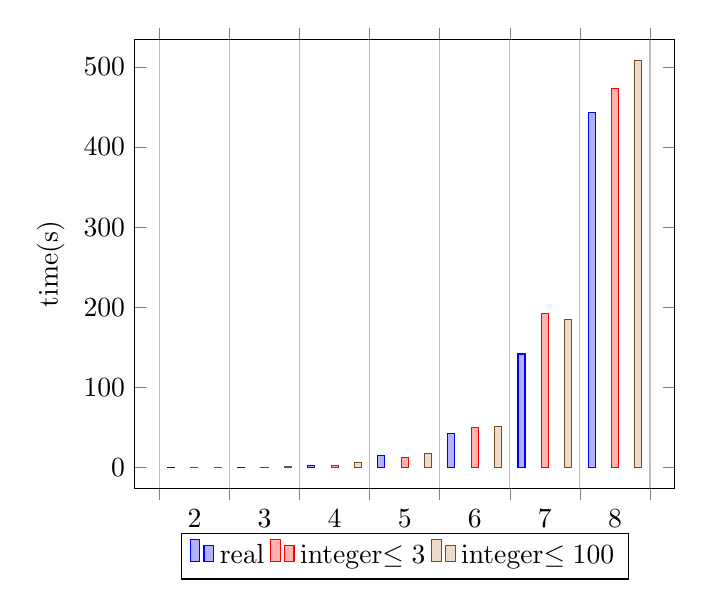
\begin{tikzpicture}
    \begin{axis}[
        xlabel= size,
        x tick label style={
            /pgf/number format/1000 sep=},
        ylabel=time(s),
        enlargelimits=0.05,
        legend style={at={(0.5,-0.1)},
        anchor=north,legend columns=-1},
        ybar interval= 0.3,
    ]
    \addplot 
        coordinates 
            {(2,0.062) (3,0.452) (4,3.258) (5,15.262) (6,43.181) (7,141.861)
             (8,442.580) (9,0)
            };
    \addplot 
        coordinates 
            {(2,0.055) (3,0.489) (4,3.191) (5,13.067) (6,49.834) (7,192.078) (8,472.704) (9,0)}; 
    % \addplot 
    % coordinates 
    %         {(2,0.074) (3,0.513) (4,3.762) (5,15.060) (6,53.805) (7,185.687) (8,571.596) (9,0)}; 
    \addplot 
    coordinates 
            {(2,0.064) (3,0.893) (4,5.966) (5,17.879) (6,50.973) (7, 184.272) (8,508.297) (9,0)}; 
    \legend{real, integer$\leq 3$,
    %  integer$\leq 10$, 
     integer$\leq 100$}
    \end{axis}
    \end{tikzpicture} 

% The time required to solve a MIP with real weights is almost the same as for solving a MIP with integer weights. The time needed to find the simple weighted type graph grows exponentially, with a factor of approximately 4, due to the increasing number of morphisms relative to the type graph size. Experiments conducted on MIPs with integer weights and different upper bounds on weights show that the upper bound has minimal influence. This justifies our choice of a mixed-integer programming solver instead of an SMT solver. Additionally, the runtime for finding a type graph of size 9 remains reasonable, whereas other implementations struggle with type graph sizes greater than or equal to 4.